  \documentclass[11pt]{article}
\usepackage[french]{babel}

\usepackage[utf8]{inputenc}
\usepackage{palatino}
\usepackage[T1]{fontenc}


\usepackage{url}
\usepackage{amsmath}

\usepackage[top=2cm,bottom=2cm,left=2.1cm,right=2.1cm,headsep=10pt,a4paper]{geometry}
\usepackage{fancyhdr}


\usepackage{graphicx,float} % figure et placement de figure
\usepackage{listings} %%inclusion de programmes
\usepackage{enumitem} 
\usepackage[french]{babel}
\frenchbsetup{StandardLists=true} 

\lstset{
  language=C++,
  basicstyle=\ttfamily\small, %
  identifierstyle=\color{black}, %
  keywordstyle=\color{blue}, %
  stringstyle=\color{blue}, %
  commentstyle=\it\color{green}, %
}

\usepackage{xcolor}

\pagestyle{fancy}
\lhead{}
\chead{\fontsize{10}{10}{Mif24 - UCBL - 2013/2014}}
\rhead{}
\lfoot{\fontsize{10}{10}{Rapport Chemier, Duhamel, Farges}}

\renewcommand{\headrulewidth}{0pt}
\renewcommand{\footrulewidth}{0pt}


 \author{\fontsize{14}{14}{\bf Aurélien CHEMIER, Arnaud DUHAMEL, Maëlyss FARGES}}
 \title{\fontsize{16}{16}{{\bf TP 1\\ Interaction multi-Agents}}}
 \date{\fontsize{11}{11}{Université Lyon 1 - 2014}}

\begin{document}

  \thispagestyle{empty}
  \maketitle
  \tableofcontents
  
  
  \newpage
  
  \section{Introduction}
  
  Le but de ce TP est de gérer des interactions entre plusieurs Agents.
  
  Pour cela les Agents sont placés sur une grille de taille n*n définissable par l'utilisateur et doivent atteindre une case "cible".
  L'objectif de l'Agent est donc d'atteindre la cible en prenant en compte les déplacements et les positions des autres Agents.
  
  \section{Implementation}
  
  Pour réaliser ce TP, nous avons utilisé Unity 4.3.2f1 qui permet de faire des représentations graphiques 3D très simplement.
  
  Chaque Agent est un thread qui agit en parallèle des autres Agents.
  Chaque Agent peut être doté d'une vitesse propre. 
  L'objectif de chaque Agent peut être n'importe quel Object de l'environnement. 
  L'Agent peut ansi courir après un autre Agent par exemple.
  
  \subsection{V1}
  C'est la  premiere version développée.
  L'Agent se déplace sur la case la plus proche de son objectif. 
  Si elle est occupée, il envoie un message à l'occupant lui demandant de se déplacer, mais aucun Agent ne gère les messages reçus.
  
  \subsection{V2}
  
  L'Agent calcule toutes les cases à parcourir en utilisant l'algorithme A*.\\
  Ensuite à chaque étape, le mouvement de l'Agent est défini selon les cases adjacentes disponibles et les messages reçus. 
  L'Agent avance vers la première case disponible suivant cette ordre :
  \begin{enumerate}
  \item L'Agent prend le prochaine case calculée par A*. Si la case est occupée, il envoie un message demandant à l'occupant de se déplacer.
  \item	L'Agent ne bouge pas sauf s'il a reçu un message lui demandant de se déplacer.
  \item Si aucun des deux cas de figure ci-dessus ne fonctionne, 
  l'Agent se déplace donc de façon aléatoire sur l'une des cases adjacentes libre et non réservée.
  \end{enumerate}
  
  \subsection{V3}
  
  Après le calcul de A*, avant même de se déplacer, les Agents vont négocier en réservant leurs chemins grâce à un contrôleur global.
  
  Chaque réservation peut engendrer un conflit sur une case. 
  Dans ces cas là, les Agents comparent la longueur du détour à faire pour chacun d'entre eux en ne passant pas par la case contestée.
  L'Agent qui a le détour le moins long laisse la case à l'autre Agent.
  
  Si la case contestée correspond à l'arrivée d'un Agent, celui laissera passer l'autre avant de retourner à sa place.
  
  Cette algorithme est en place, mais n'a pas pu être débuggé.

  \section{Score}
  
  Une fois arrivé, chaque Agent obtient un score calculé en fonction de sa performance.
  Un score général est également calculé.
  
  \subsection{Score individuel}
  
  Le score individuel est calculé de la façon suivante:   
  \begin{math} \frac{nombre de pas minimun}{nombre de pas fait} * 100\end{math} 
  
  Le nombre de pas minimum est déterminé par le premier A* effectué en début de parcours. 
  Ce nombre de pas minimum ne prend donc 
  De plus, on peut déplacer les Agents pendant l'exécution du programme et les mettre en pause.pas en compte toutes les interactions à faire avec les autres Agents. 
  Il s'agit du nombre de pas à faire si l'Agent n'était jamais bloqué.
  
  \subsection{Score général}
  
  Le score général est calculé de la façon suivante: 
  \begin{math} \sum scores individuels\end{math} 
  
  
  \section{Exemples}
  
  \subsection{Exemple Simple}
  
   \begin{figure}[H]
      \centering
      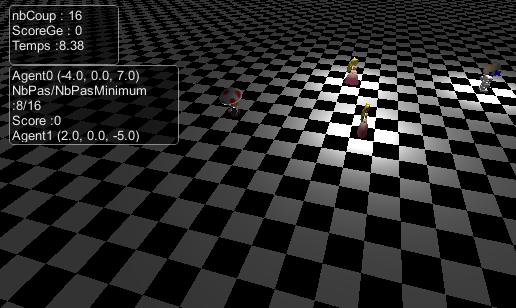
\includegraphics[scale=0.7]{Image/grandTableau.png} 
      \caption{Position de départ}
      \label{fig:grandTableau}
  \end{figure}
  
  \begin{figure}[H]
      \centering
      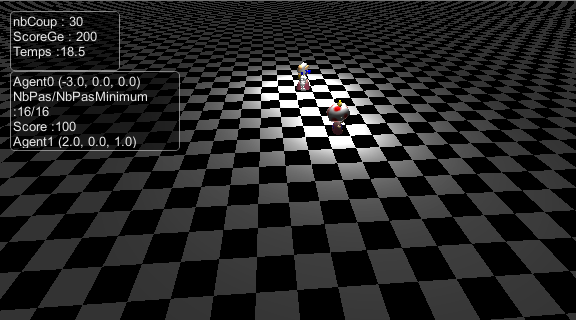
\includegraphics[scale=0.7]{Image/grandTableauSolution.png} 
      \caption{Position d'arrivée}
      \label{fig:grandTableauSolution}
  \end{figure}
  Sur cette première image, Toad et Mario sont deux Agents dont leurs objectifs est de rencontrer Peach.
  Ici, l'arène est volontairement immense (100*10) pour prouver que l'algorithme tient sur une grande grille.
  A chaque itération, Mario et Toad vont avancer vers leurs objectif respectif sans encombre.
  Dans la figure \ref{fig:grandTableauSolution}, les deux Agents ont complété leurs objectifs. 
  
  En haut à gauche est affiché le nombre de coup totaux, le score général et le temps depuis le lancement de l'application.
  En dessous est affiché pour chaque Agent : sa position, son nombre de pas actuels / le nombre de pas minimum calculé par A* sans tenir compte des obstacles Agent en début de parcours ainsi que son score.
  
  Dans notre premier exemple, nos deux Agents atteignent leur objectif sans encombre et obtiennent 100 points chacun pour un score général de 200 points en 30 coups et 18.5 secondes (l'imprime-écran n'a pas eu lieu au moment précis de la rencontre, sinon le temps aurai été de 16 secondes : 1 seconde par pas).
  
  
  
  \subsection{Exemple \'Echiquier}
  
   \begin{figure}[H]
      \centering
      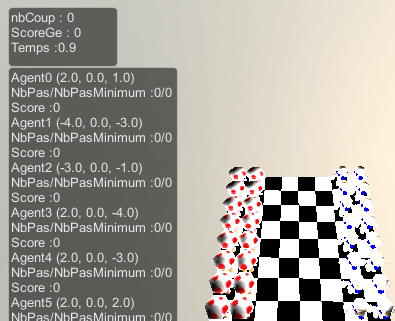
\includegraphics[scale=0.7]{Image/echequierDebut.png} 
      \caption{\'Echiquier initial}
      \label{fig:échiquierDebut}
  \end{figure}
   
  
  Nous simulons ici un échiquier où les Toad et les Mario vont échanger leur place. 
  Cette grande simulation est l'opportunité de montrer de très nombreuses négociations serrées.
  Dans la figure \ref{fig:échiquierDebut} qui se situe à t = 0 secondes, nous avons de chaque coté les deux équipes prêtent à échanger leurs places.
  
   \begin{figure}[H]
      \centering
      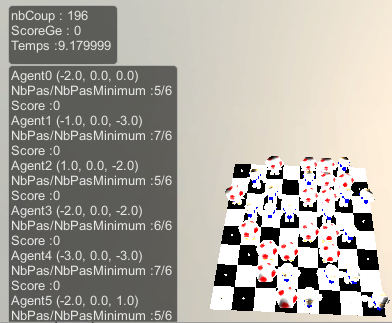
\includegraphics[scale=0.7]{Image/echequierBattle.png} 
      \caption{\'Echiquier en cours d'échange}
      \label{fig:échiquierBattle}
  \end{figure}
  
   À t = 9 secondes , les deux camps sont en plein échange de place au milieu de l'arène (figure \ref{fig:échiquierBattle}).
  Chaque Agent doit négocier avec son voisin pour avancer, tout en gérant les messages reçus de ceux qui ont réservé des places adjacentes.
  
  
   \begin{figure}[H]
      \centering
      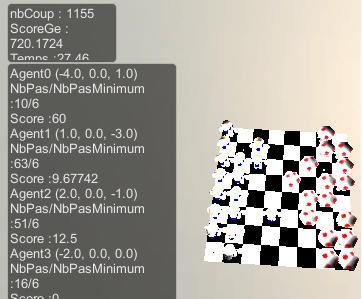
\includegraphics[scale=0.7]{Image/echequierBattlePresqueResolu.png} 
      \caption{\'Echiquier presque terminé}
      \label{fig:échiquierBattlePresqueResolu}
  \end{figure}
  
  
  Après un peu plus de 20 secondes de négociation les Toads et les Marios on échangé leurs places (figure \ref{fig:échiquierBattlePresqueResolu}).
  Viens la deuxième épreuve : le placement de l'autre coté de la grille. En effet, si un Agent se place correctement il risque de bloquer le passage à un autre Agent. 
  En se déplaçant, ce premier Agent risque à nouveau de bloquer un autre Agent et ainsi de suite.
  Si les Agents sont bloqués, ceux-ci se déplacent aléatoirement autour d'eux, ainsi au bout d'un certain temps il est certain que chacun trouvera sa place.
  
  
   \begin{figure}[H]
      \centering
      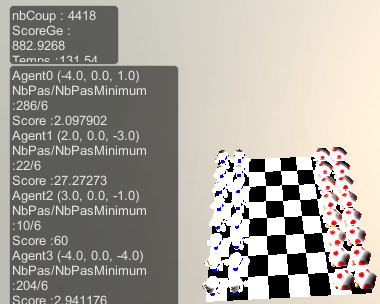
\includegraphics[scale=0.7]{Image/echequierBattleResolu.png} 
      \caption{\'Echiquier à la fin}
      \label{fig:échiquierBattleResolu}
  \end{figure}
  
  A t = 130 secondes, tout les Agents ont échangé leurs positions. L'expérience est un succès !
  On constate que quelques Agents ont trouvé leur emplacement en peu de déplacements (Agent 1 avec seulement 22 déplacements) tandis que d'autre ont dû être énormément sollicité (Agent 0 avec 286 déplacements).
  Les Agents peu sollicités doivent être ceux disposé aux coins de l'arène, tandis que les autres sont ceux posé en plein milieu, source de beaucoup de gènes pour les autres Agents et sont donc ceux qui ont besoin de beaucoup de négociations.
  
  \subsection{Autres exemples}
   Tout les exemples présenté et bien d'autres sont des scènes chargeable depuis Unity.
   \begin{itemize}
   \item Scénario 1 met en scène plusieurs Agents avec un même objectif. 
   \item Scénario 2 oblige un Agent à éviter un mur pour passer. 
   \item Scénario 3 met en scène un unique chemin que deux Agents doivent emprunter. 
   Il vont devoir négocier pour savoir lequel des deux passera en premier. 
   \item Scénario 4 met en scène un labyrinthe ou plusieurs Agents vont passer les uns après les autres pour rejoindre leur objectif personnel.
  \end{itemize}
  
  \section{Conclusion}
  
  Ce système simple d'Agents semble marcher pour tous les cas de figure.
  Les nombreux paramètre des Agents sont facilement modifiable via l'interface d'Unity (figure \ref{fig:unity}). On peut ainsi modifier la vitesse d'un Agent et son objectif par exemple grâce à la fenêtre Inspector de droite.
 
 On peut aussi ajouter des "murs" en rendant un Agent "sourd" au messages en cochant Stategie Agent Bloquant dans l'Inspector. 
  Un tel Agent ne se déplacera pas en fonction des autres Agents, mais au contraire leurs répondra qu'il ne compte pas bouger, les forçant à trouver un autre chemin.
  
  
  De plus, on peut déplacer les Agents pendant l'exécution du programme et les mettre en pause.
  
  \begin{figure}[H]
      \centering
      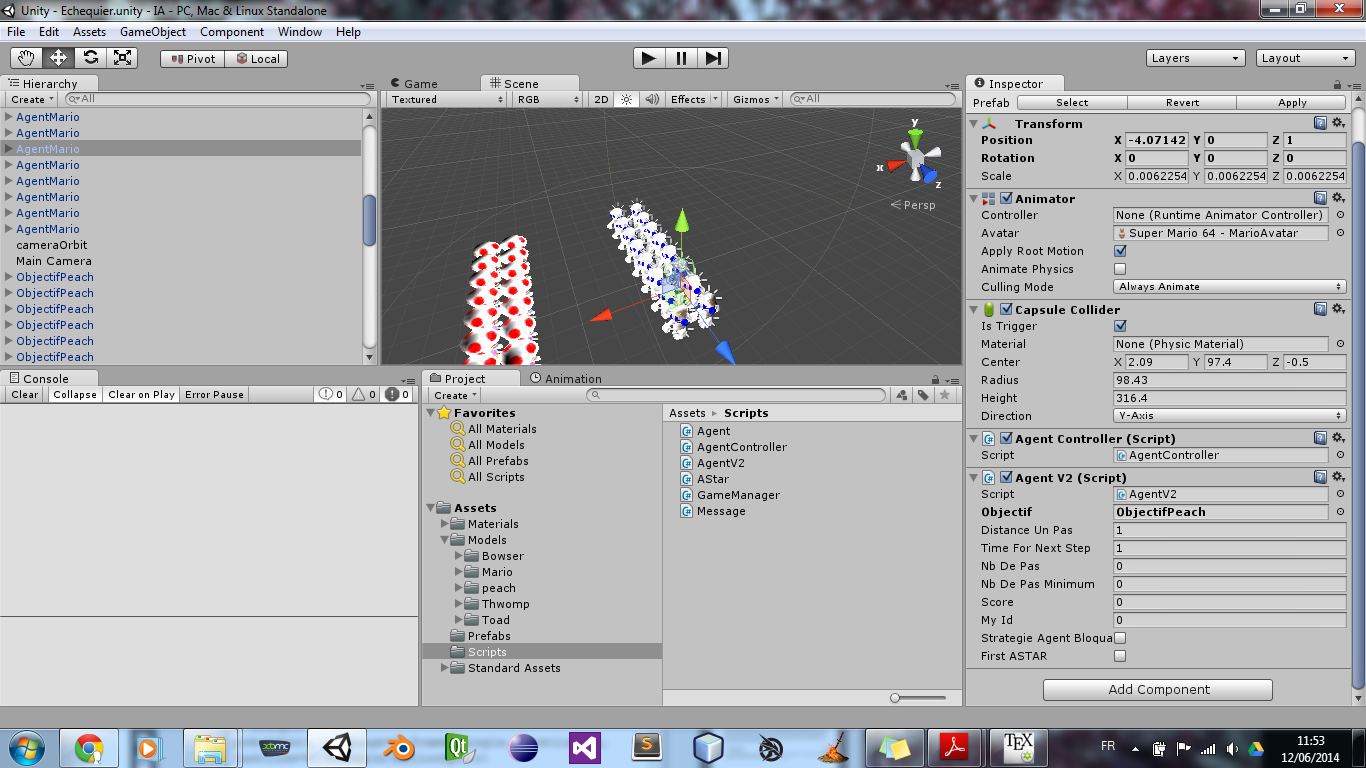
\includegraphics[scale=0.4]{Image/unity.png} 
      \caption{Interface Unity}
      \label{fig:unity}
  \end{figure}
  
  
  Même si l'Agent V3 n'a pas pu être terminé, cette implémentation offre d'ores et déjà une interface intuitive et une IA simple et efficace dans la résolution de chemin Multi-Agents. 
  

  
  \end{document}
%\lstinputlisting[caption={Exemple de pointeur constant},language=C,frame=single]{Exemple/pointeurConstant.c}
%  \lstinputlisting[caption={Optimisation de l'exemple précédent},language=C,frame=single,firstline=6, lastline=6]{Exemple/mallocOpt.c}

 %\begin{figure}[H]
 %      \centering
  %     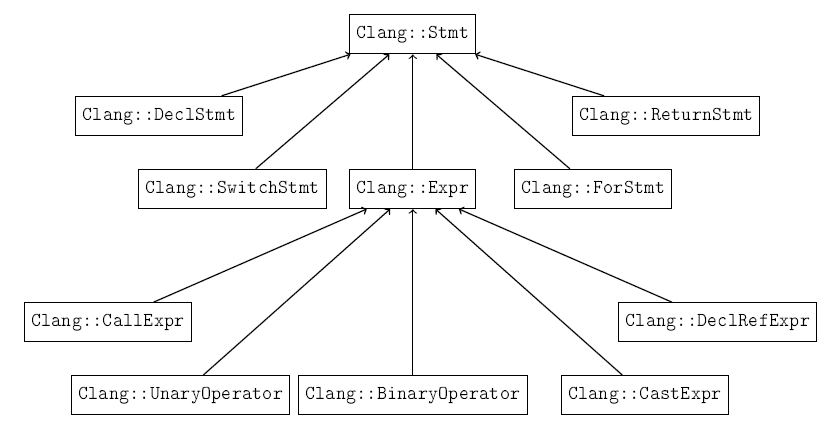
\includegraphics[scale=0.7]{soluce/graph.jpg} 
 %      \caption{Partie de l'architecture de Clang}
  %     \label{fig:graph}
  %   \end{figure}